\documentclass[12pt, twoside]{article} 
\newcommand{\hdir}{.}
\usepackage{./jmlda}
%\usepackage[round]{natbib}
\usepackage[square,sort,comma,numbers]{natbib}
\usepackage{rotating}
\usepackage{tabularx} % for 'tabularx' env. and 'X' col. type
\setlength\extrarowheight{2pt} % make the tables look less cramped
\usepackage{hyperref}
\usepackage{graphics}
\usepackage{wrapfig}
\usepackage{comment}
\usepackage{multicol}
\usepackage{graphicx}
% теоремы
\newtheorem{theorem_takkens}{Таккенс \cite{takkens}}
\newtheorem{def_1}{Динамическая система}

\begin{document}
\title
	[Детекция зависимостей во временных рядах]
	{Детекция зависимостей во временных рядах}
\author
	[I. M. Latypov]
	{I. M. Latypov, E. Vladimirov, V. V. Strizhov}
\email
	{latypov.im@phystech.edu}
\organization	
	{MIPT}	
\abstract
	{
		Для многих прикладных задач \cite{Averta2021}\cite{Camargo2021}\cite{Higuchi1999} требуется решать задачу выявления зависимостей между временными рядами. 
		Выявление этих зависимостей и их последующее использование направлено на то, чтобы улучшить качество модели. В статье для обнаружения подобных зависимостей предлагается использовать *модели пространства состояний*. Приведен пример использования метода на основе скрытых состояния модели ODE-RNN \cite{Rubanova2019}. Скрытые состояния рассматриваются как представление временного ряда, и после этого к ним примяется метод сходящегося перекрестного отображения (Convergent Cross Mapping) \cite{Sugihara2012}.
		
	%	При прогнозировании временных рядов, зависящих от других временных рядов, требуется решить задачу выявления связей между ними.
	%	Предполагается, что добавление связанных временных рядов в прогностическую модель повысит качество прогноза. В данной работе для
	%	обнаружения зависимостей между временными рядами предлагается совместить Convergent Cross Mapping с ODE-RNN. 
		}
\bigskip
\noindent

\maketitle
\textbf{Ключевые слова}: \emph{временные ряды, CCM, ODE-RNN, Neural ODE}

\section{Введение}
		Решается задача поиска причинно-следственных связей между временными рядами. На практике у изучаемой динамической системы несколько наблюдаемых величин,
		 измерения которых представляют собой временной ряд. 
		Исследование этих рядов входит в состав задачи исследования системы. Выявление причинно-следственных взаимосвязей между временными рядами наблюдаемых величин рассматривается -- важная часть исследования временных рядов. Например на основе анализа зависимости временных рядов данных гироскопов у танцующей пары можно делать выводы о качестве их взаимодействия.
		
		%	Наша цель - развить идею метода сходящегося перекрестного отображения. Изначально этот метод является непараметрическим, мы показываем что можно приме
		% Далее в разделе \hyperref[sec:math_form]{<<математическая постановка>>} привелена строгая постановка задачи и предлагаемый метод решения. В разделе \hyperref[sec:theor_background]{<<теоритичесие предпосылки>>} приведены теоритические предпосылки на которых основывается предлагаемый метод. 
		
\section{О подходах к решению задачи}	
%\label{sec: related_works}
	
	Кросс Корреляция -- метод проверяет коррреляцию временных рядов при из сдвигах. Зависимость оценивается на основе максимальной полученной корреляции.
	
	Тест Гренжера \cite{Granger1980} - на паре временных рядов обучаются две модели: первая обучается предсказвать первый временной ряд  только на данных этого ряда. Вторая тоже обучается предсказвыать первый временной ряд, но уже на данных обоих временных рядов. Если качество предсказаний на второй модели существенно возрастает, то делается вывод о зависимости временных рядов.
	
	 Кластеризация квазипериодических временных рядов \cite{A.V.Grabovoy2018} -- использование метода главных компонент с новой метрикой. 
	 
	 \cite{Kwapisz2010} -- описывает метод построения описания объекта на основе экспертно определенных генерирующих функций.
	
	Метод перекрестного сходящегося отображения \cite{McCracken2014} будет рассмотрен далее в деталях как основа для построения нашего метода.
	
	Общим недостатком для всех методов является квадратичное от длительности наблюдений время работы. Другие достоинства и недостатки некоторых методов можно посмотреть в таблице 1.
	
\newpage

\begin{table}[h!]
	\caption{Сравнение методов}
	\begin{tabular}{|l|l|l|}
		\hline
		Метод                                                                  & Достоинства                                                                                                            & Недостатки                                                                                                                                                 \\ \hline
		Тест Грэнджера \cite{Granger1980}                     & \begin{tabular}[c]{@{}l@{}}Анализ рядов совмещается\\ с построением модели \\ предсказания.\end{tabular}               & \begin{tabular}[c]{@{}l@{}}Не дает представлений\\ о виде зависимости рядов. \\ Предсказания могут не \\ улучшиться из-за \\ неверной модели.\end{tabular} \\ \hline
		Кросс Корреляция \cite{Yoo2009}                       & \begin{tabular}[c]{@{}l@{}}Не  требуется дополнительная \\ обработка данных\end{tabular}                               & \begin{tabular}[c]{@{}l@{}}Корреляция не является \\ достаточным условием \\ зависимости.\end{tabular}                                                     \\ \hline
		CCM \cite{Sugihara2012}                              & \begin{tabular}[c]{@{}l@{}}Возможна работа с более \\ сложными зависимостями \\ чем в предыдущих методах.\end{tabular} & \begin{tabular}[c]{@{}l@{}}Ислледование \cite{McCracken2014} \\ выделяет недостатки.\end{tabular}                                         \\ \hline
		\begin{tabular}[c]{@{}l@{}}CСM + ODE-RNN\\ (предлагаемый)\end{tabular} & \begin{tabular}[c]{@{}l@{}}Применяется к многомерными\\ временными рядам.\end{tabular}                                 & \begin{tabular}[c]{@{}l@{}}Так как метод \\ параметрический, его \\ нужно обучать на \\ исследуемых данных.\end{tabular}                                \\ \hline
	\end{tabular}
\end{table}
			
	
\section{Математическая постановка}
\label{sec:math_form}

Обозначим $T = \{t_1, ... t_k\}$ - моменты наблюдений. И введем обозначения 

$$\mathbf{x} = \{\mathbf{x_1}, \mathbf{x_2}, ... \mathbf{x_k}\} , \mathbf{y} = \{\mathbf{y_1}, \mathbf{y_2}, ... \mathbf{y_k}\}$$

  наблюдения за парой многомерных временных рядов. $x_i \in \mathbb R^m$, $y_i \in \mathbb R^n$,   в работе опыты проводятся при $m = n = 3$. Наблюдения $x_i, y_i$ сделаны в момент $t_i$. Промежутки между наблюдениями одинаковы, то есть частота семплирования рядов постоянна.

Ставится задача построения отображения $\phi : \{\mathbf x  \times \mathbf y \} \rightarrow \mathbb{R}$ по значениям которой будет делаться вывод о зависимости временных рядов.

\section{предлагаемый метод}
	В качестве основы для модели берется метод сходящегося перекрестного отображения, поэтому рассмотрим его подробно. Метод применяется для пары одномерных временных рядов $\mathbf{x} = [x_1 , ..., x_N]$  и $\mathbf{y} = [y_1, ..., y_N]$. Индексирование такое же как в \hyperref[sec:math_form]{\textbf{постановке}}. Идея метода основана на теореме Таккенса \cite{takkens}. Теорема утверждает, что для временного ряда, представляющего собой наблюдения за динамической системой и удовлетворяющего перечисленным выше условиям -- а именно для рядов с постоянной частотой семплирования, по векторам $[x_i, x_{i+1}, ..., x_{L -1}]$ строится изоморфизм в прострванство, в котором развивается динамическая система. То есть такие вектора описывают динамическую систему. Здесь $L$ - размерность отображения. Далее будем называть это размерностью погружения. Согласно этой теореме должно быть выполнено $L \geq 2m$, где $m$ - истинная размерность системы. На практике $m$ нам не известно. 
	
	Метод рассматривает отображение временных рядов в траекторное подпространство с матрицей Ганкеля временного ряда и оценивает, насколько хорошо траектория эволюции одного ряда восставнавливается по траекторий эволюций другого. Опишем как это делается. Для рядов строится матрица Ганкеля:
	$$
	\mathbf{H}_{x} =
	\left( {\begin{array}{ccccc}
			x_1 & x_2 & ... & x_{L-1} & x_L\\
			x_2 & x_3 & ... & x_{L} & x_{L +1}\\
			... & ... & ... & ...   & ... \\
			x_{N-L+1} & x_{N-L +2} & ... & x_{N-1} & x_N\\
	\end{array} } \right)
	$$
	$L$ - размерность погружения, используемая для построения отображения в пространство эволюции системы. Так же строится матрица Ганкеля второго ряда $\mathbf{H}_y$.
	Обозначим через $\mathbf{x}_{t}$ $t - L$-ую строку $H_x$, $\mathbf{y}_{t}$ $t - L$-ую строку $H_y$. Тогда вектора $\mathbf{x}_t$ рассматриваются как точки в траекторнорм пространстве $\mathbf{M}_x$, $\mathbf{y}_t$ - как точки в траекторнорм пространстве $\mathbf{M}_y$. В этих пространствах выбирается евклидова метрика.
	Для восстановления измерения $y$ в момент времени $t\in L + 1,..., N$ найдем $k$ ближайших соседей вектора $\mathbf{x}_t$. Обозначим их по возрастанию расстояния до $\mathbf{x}_t$:
	$$[\mathbf{x}_{t_1}, \mathbf{x}_{t_2}, ...,\mathbf{x}_{t_k}]$$. 
	$\mathbf{x}_{t_k}$ -- самый дальний их $k$ соседей. После этого строится прогноз $y_t$ следующим образом:
	$$
	y^t = \sum^k_{i = 1}w_iy_{t_i}$$
	Где
		$$	w_i = \frac{u^i}{\sum_i u_i}, \qquad u_i = \exp\bigg(-\frac{\|\mathbf{x_t} - \mathbf{x_{t_i}}\|_2}{\|\mathbf{x_t} - \mathbf{x_{t_k}}\|_2}\bigg)
	$$
	
	
	Для обнаружения зависимости рядов рассматривается корреляция между предсказаниями и значениями ряда. На основании величины корреляции делается вывод о зависимости или независимости рядов.
	
	Чтобы развить этот метод рассмотрим параметрическое построение погружений. Для этого обратимся к моделям пространства состояний -- моделям дискретного описания динамической системы. При таком подходе совсместно с временным рядом рассматривается дополнительный вектор скрытых состояний, который эволюционирует совместно с наблюдениями за системой.
	
	В самом простом виде уравнения развития скрытых состояний системы можно задать как два уравнения эволюции. Вектор скрытых состояний системы $u$, вектор наблюдений за системой $x$ и уравнения:
\begin{equation}
	\begin{split}
		u_t = F(u_{t-1}, y_t) \\ 
		z_{t} = G(u_t, y_t)
	\end{split}
\end{equation}
Здесь $z$ -- моделируемая величина. Второе уравнение нам не нужно, так что далее рассматриваем только первое, из которого получаются скрытые состояния.

Итоговая модель выглядит просто:
\begin{equation}
	\begin{split}
		u_0 = f(x_0) \\ 
		u_{k + 1} = \psi(u_k, x_k)
	\end{split}
\end{equation}
Мы выделили два различных способа задания функции $\psi$ -- непрерывное и дискретное и рассмотрели их в экспериментах. Дискретное изменение моделирорвалось с помощью GRU модуля. Для моделирования непрерывных изменений была взята модель ODE-RNN \cite{Rubanova2019}, 

ODE-RNN строится на последовательном применении - Neural ODE \cite{Chen2018} и RNN.
В качестве $u_i$ -- используются скрытые состояния RNN модуля. В моменты наблюдений скрытое состояние меняется с RNN $u_{t_i} = RNN(\widetilde{u_{t_i}}, x_{t_i})$, затем полученное скрытое состояние эволюционирует к следующему моменту времени с NeuralODE: $u_{t_{i+1}} = \text{ODESolve}(f_\theta, u_{t_i}, (t_i, t_{i+1}))$. Здесь $f_\theta$ -- уравнение использующееся в качестве дифференцциального уравнения. $\text{ODESolve}$ -- вызов Neural ODE. Видно, что модель работает независимо от промежутков между семплированими. 

\section{Вычислительные эксперименты}
\label{experiments}


\begin{wrapfigure}{r!}{0.4\textwidth}
	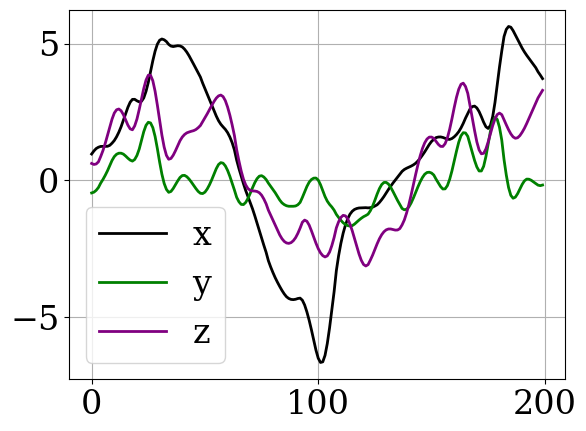
\includegraphics[width=0.4\textwidth]{images/ряд.jpg} 
	\caption{Ряд значений показаний гироскопа на отрезке в 250 семплов}
	\label{ряд}
\end{wrapfigure}

	Кратко опишем выбрку на которой проводились эксперименты. Данные представляют собой записи показаний акселерометра и гироскопа при ходьбе и при беге на протяжении 30 -- 40 секунд. За это время делается примерно 15 движений. Частота семплирования равна 200 Гц. Датчики находятся на концах рук, так что можем рассматривать пары временных рядов и применять к ним метод. Можно посмотреть пример временного ряда гироскопа на картинке \ref{ряд}.

\begin{wrapfigure}{r!}{0.4\textwidth}
	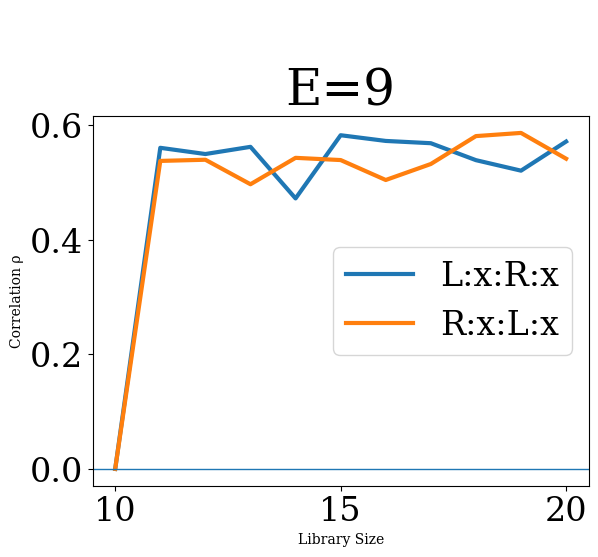
\includegraphics[trim={0.6cm 0.8cm 0 2.7cm},clip=true,width = 0.4\textwidth]{images/method_3d.jpg}
	\caption{ODE-RNN + CCM  для правого и левого гироскопа на трехмерных данных. Оси: ox -- количество опорных точек метода CCM, oy -- корреляция, получаемая при применении метода}
	\label{method_apply_rez}
\end{wrapfigure}

	Сначала посмотрим на работу метода на паре одномерных временных рядов. В качестве функции $\psi$ используется ODE-RNN. Отрисуем траектории скрытых состояний временных рядов в скрытых состояниях, которые получаются методом CCM. Для этого из погружений рядов -- матрицы Ганкеля выделяются главные компоненты. Подробнее в работе \cite{Usmanova2018}. Для наглядности траектории были спроецированы на сферу.
	
	В предложенном методе матрица скрытых состояний получается не ганкелевой, поэтому к ней перед построением траекторий применяется метод многомерной гусеницы (анализ сингулярного спектра) \cite{SSA1997}
	Результаты можно увидеть на рис. \ref{trajectory_CCM} и \ref{trajectory_hidden}.
	
	
	То есть в скрытых состояниях появляются одинаковые периодические структуры. Применим метод CCM к скрытым состояниям. Для сравнения приведен результат применения CCM к самим временным рядам. Результаты можно увидеть на рис. \ref{CCM_apply}.



Видно что на рассматриваемых данных предложенный метод так же выделяет зависимость.
Как отмечалось ранее - наблюдения на датасете с акселерометром - трехмерные, и предложенный метод создается чтобы работать именно с такими данными. Посмотреть траектории скрытых состояний и результат применения метода к данным можно на рис. \ref{method_apply_rez} и \ref{method_apply}.


\section{анализ свойств предложенного метода}
\label{sec:theor_background}

Из рисунка \ref{trajectory_hidden} видно, что траектории предложенного метода совпадают не так хорошо как у CCM. Это происходит из-за того, что модель параметрическая. ODE-RNN обучаются на разных данных, и поэтому достигаются разные локальные минимумы. 

Следующий важный гиперпараметр при подготовке модели - количество этох для тренировки. При экспериментах модель обучалась 9 эпох. Если обучение длится мало, то корреляция снижается, а траектории сильно отличаются. Если же модель переобучается, то траектории становятся хаотичными и корреляция соответственно значительно уменьшается.

Так же важна размерность погружения. Если взять слишком большую размерность, то корреляция начинает уменьшаться. На это предположительно есть две причины. Первая связана с проклятием размерности -- евклидова метрика плохо работает на большиз размерностях. Вторая -- модель слишком сложная для рассматриваемых данных, из-за чего некоторое подмножество весов плохо обучается.

\section{Заключение}

Предложили метод для выявления взаимной зависимости временных рядов.  В отличие от других популярных методов его можно применить к многомерным данным. К тому же метод является параметрическим. Это и достаток метода -- после обучения выявляются более глубокие признаки данных, и его недостаток -- необходимо подбирать параметры и обучать модель.

   Опыты показали, что метод работает с парой измерений датчиков на теле так же как и CCM. Кроме того и одномерные, и многомерные данные погружаются в структуры, похожие на погружения при методе CCM. То есть информация о периодичности рядов, их частоте и другие данные сохраняются при погружении.
   
   Границы применимости метода пока что открытый вопрос.


\section{Список литературы}

\bibliographystyle{plain}
\bibliography{library.bib}

\newpage
\section{картинки}
\begin{figure}[h!]
	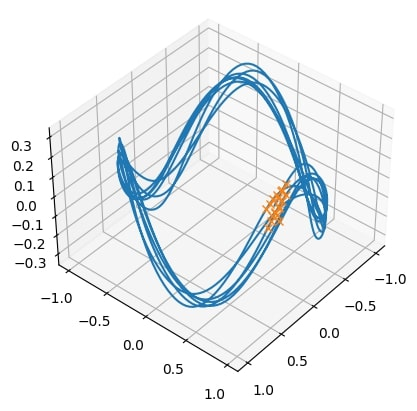
\includegraphics[width = 0.5\textwidth]{images/trajectory_CCM.jpg} \hfill
	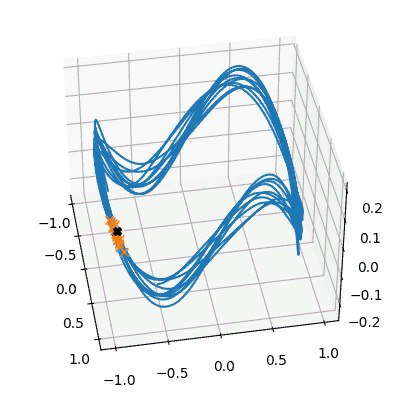
\includegraphics[width = 0.5\textwidth]{images/trajectory_CCM_right.jpg}
	\caption{слева направо - траектория скрытых состояний при использовании CCM левого/правого гироскопа на одномерных данных}
	\label{trajectory_CCM}
\end{figure}	


\begin{figure}[h!]
	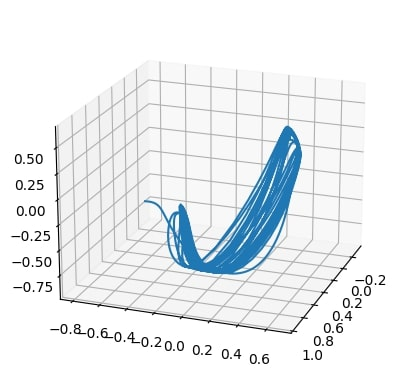
\includegraphics[width = 0.5\textwidth]{images/trajectory_left.jpg} \hfill
	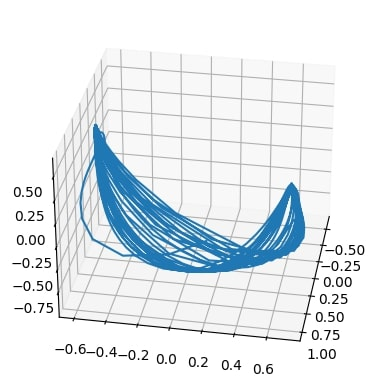
\includegraphics[width = 0.5\textwidth]{images/trajectory_right.jpg}
	\caption{слева направо - траектория скрытых состояний при использовании ODE-RNN + гусеница левого/правого гироскопа на одномерных данных}
	\label{trajectory_hidden}
\end{figure}	


\begin{figure}[h!]
	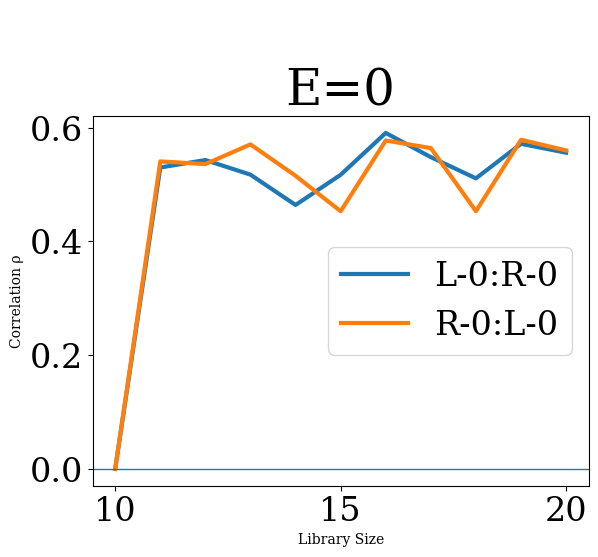
\includegraphics[trim={0.6cm 0.8cm 0 2.7cm},clip=true,width = 0.5\textwidth,height=0.3\textheight]{images/CCM_experiments/net_exp.jpg} \hfill
	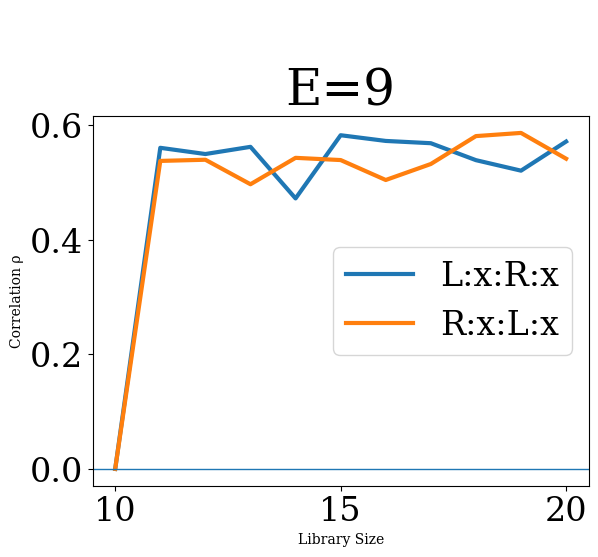
\includegraphics[trim={0.6cm 0.8cm 0 2.7cm},clip=true,width = 0.5\textwidth,height=0.3\textheight]{images/CCM_experiments/CCM_exp.jpg} 
	\caption{слева направо: ODE-RNN + CCM / CCM для правого и левого гироскопа на одномерных данных. Оси: ox -- количество опорных точек метода CCM, oy -- корреляция, получаемая при применении метода}
	\label{CCM_apply}
\end{figure}

\begin{figure}[h!]
	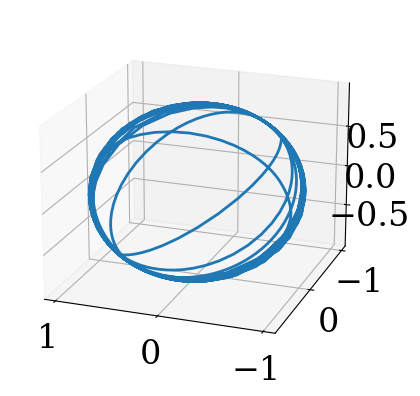
\includegraphics[width = 0.5\textwidth,height=0.3\textheight]{images/left_3d.jpg} \hfill
	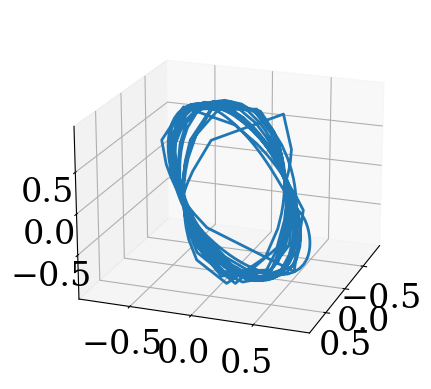
\includegraphics[width = 0.5\textwidth,height=0.3\textheight]{images/right_3d.jpg} 
	\caption{слева направо - траектория скрытых состояний при использовании ODE-RNN + гусеница левого/правого гироскопа на трехмерных данных}
	\label{method_apply}
\end{figure}






\end{document}